\documentclass[a4paper]{article}

\usepackage[utf8]{inputenc}
\usepackage[T1]{fontenc}
\usepackage{textcomp}
\usepackage[english]{babel}
\usepackage{amsmath, amssymb}


%figure support
\usepackage{import}
\usepackage{xifthen}
\pdfminorversion=7
\usepackage{pdfpages}
\usepackage{transparent}
\newcommand{\incfig}[1]{%
	\def\svgwidth{\columnwidth}
	\import{./figures/}{#1.pdf_tex}
}
\graphicspath{ {./figures/} }
\pdfsuppresswarningpagegroup=1

\begin{document}
	\title{EEL4768C.04 Homework 4 Due 10/27/19}
	\author{Brandon Thompson 5517}
	\maketitle

	\begin{enumerate}
		\item Modify the single-cycle MIPS processor to implement the \texttt{jal}
			instruction. See Appendix B for a definition of the instruction.
			Mark up a copy of Figure \ref{fig:1cycle_processor} to indicate the changes
			to the datapath. Name any new control signals. Mark up a copy of
			Table \ref{tab:dec_truth_table}
			to show changes to the main decoder. Describe any other changes
			that are required.\\
			\\
			26-bit immediate must be extracted and shifted 2 bits to the left to create
			a 28-bit number. To create a 32-bit PC, the top 4 bits of the current PC are
			merged in. The PCSrc multiplexor need to be extended with a third input.\\
			The return address (\texttt{PC+4}) needs to be routed to the \texttt{WD3}
			port of the register file. Extended the \texttt{MemtoReg} mux.\\
			Return address needs to be written to register 31, 31 must be hard coded
			into the \texttt{RegDst} mux.
			\begin{figure}[ht]
				\centering
				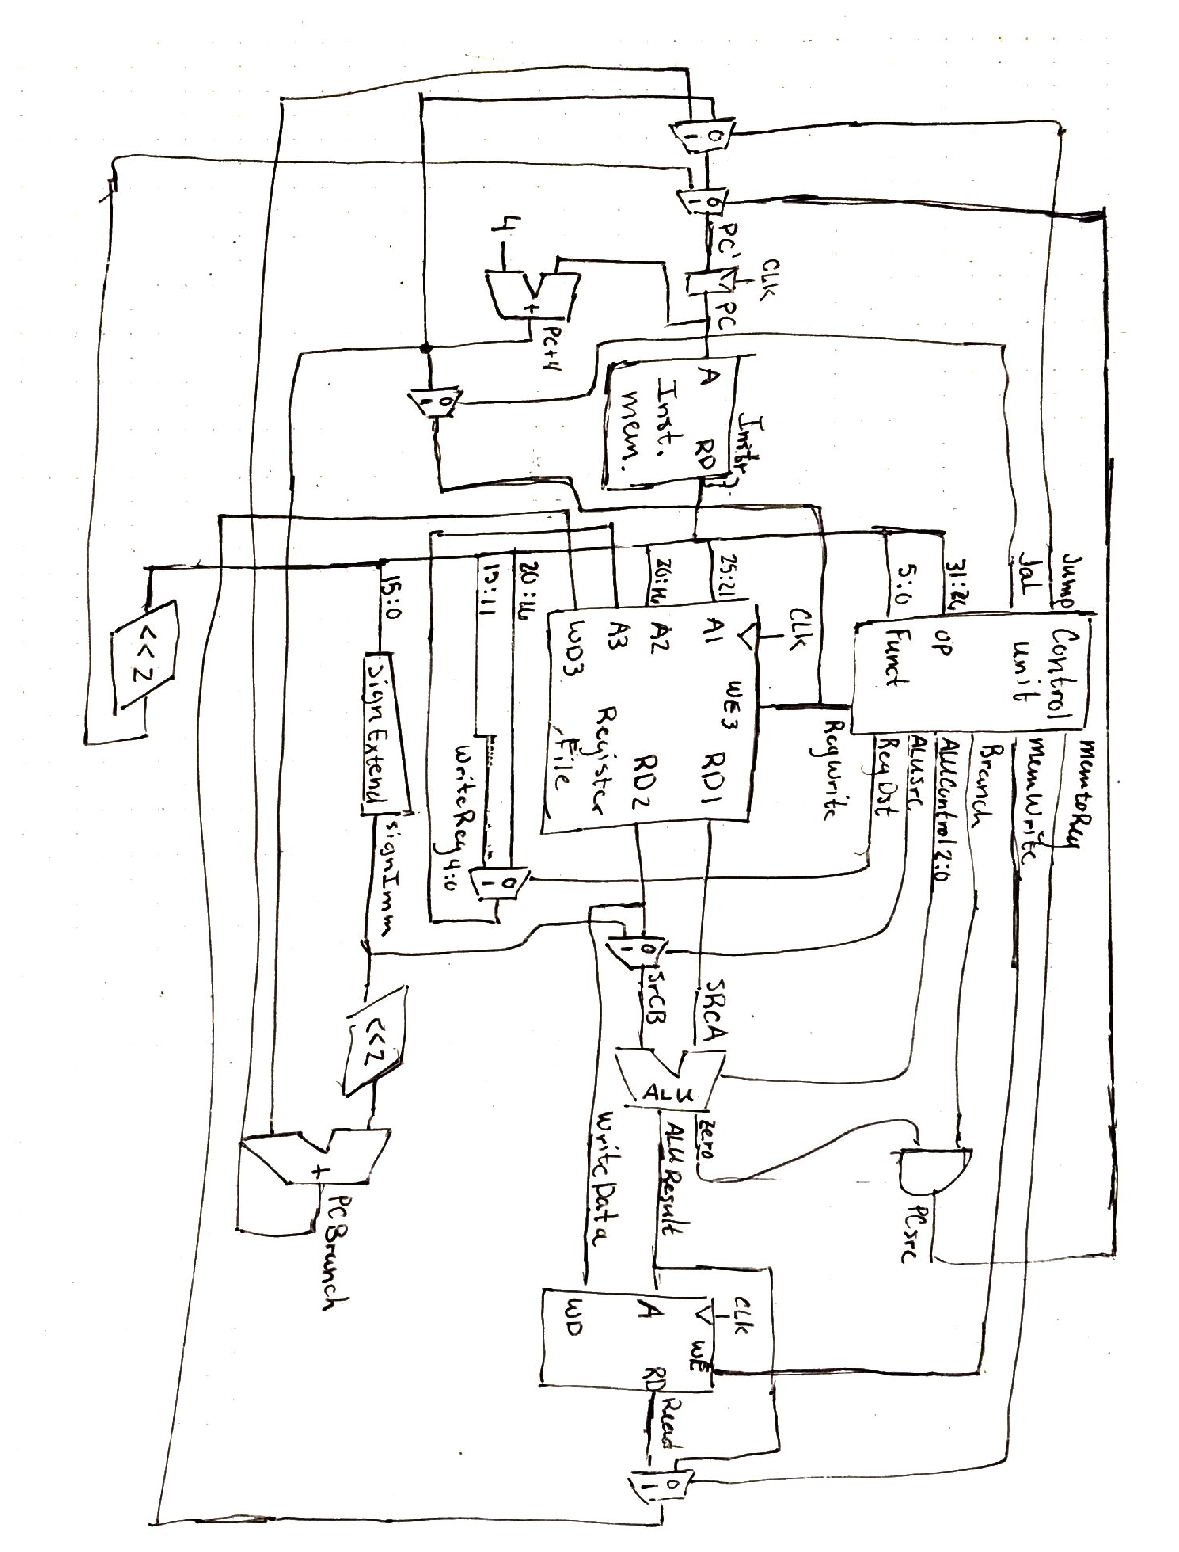
\includegraphics[angle=90,origin=c,width=0.8\textwidth]{7_4a}
				\caption{MIPS single-cycle processor with \texttt{jal} instruction.}
				\label{fig:7_4a}
			\end{figure}
			\begin{table}[ht]
				\noindent\makebox[\textwidth]{
				\begin{tabular}{| c c c c c c c c c |}
				\hline
				Instruction & Opcode & RegWrite & RegDst & ALUSrc & Branch & MemWrite & MemtoReg & ALUOp\\
				\hline
				\hline
				R-Type & 000000 & 1 & 1 & 0 & 0 & 0 & 0 & 10\\
				\hline
				\texttt{lw} & 100011 & 1 & 0 & 1 & 0 & 0 & 1 & 00\\
				\hline
				\texttt{sw} & 101011 & 0 & X & 1 & 0 & 1 & X & 00\\
				\hline
				\texttt{beq} & 000100 & 0 & X & 0 & 1 & 0 & X & 01\\
				\hline
				\texttt{jal} & 000011 & 1 & X & 1 & 0 & 0 & X & 00\\
				\hline
				\end{tabular}
                		}
			\caption{Decoder truth table for \texttt{jal} instruction.}
        		\label{tab:jal_truth_table}
        		\end{table}
			\pagebreak
		\item Repeat for \texttt{jr} instruction.
			Expand \texttt{PCSrc} mux for another input, \texttt{JmpReg} from control
			unit is used to determine output. \texttt{RD1} is used as input to the mux.
			\begin{figure}[ht]
				\centering
				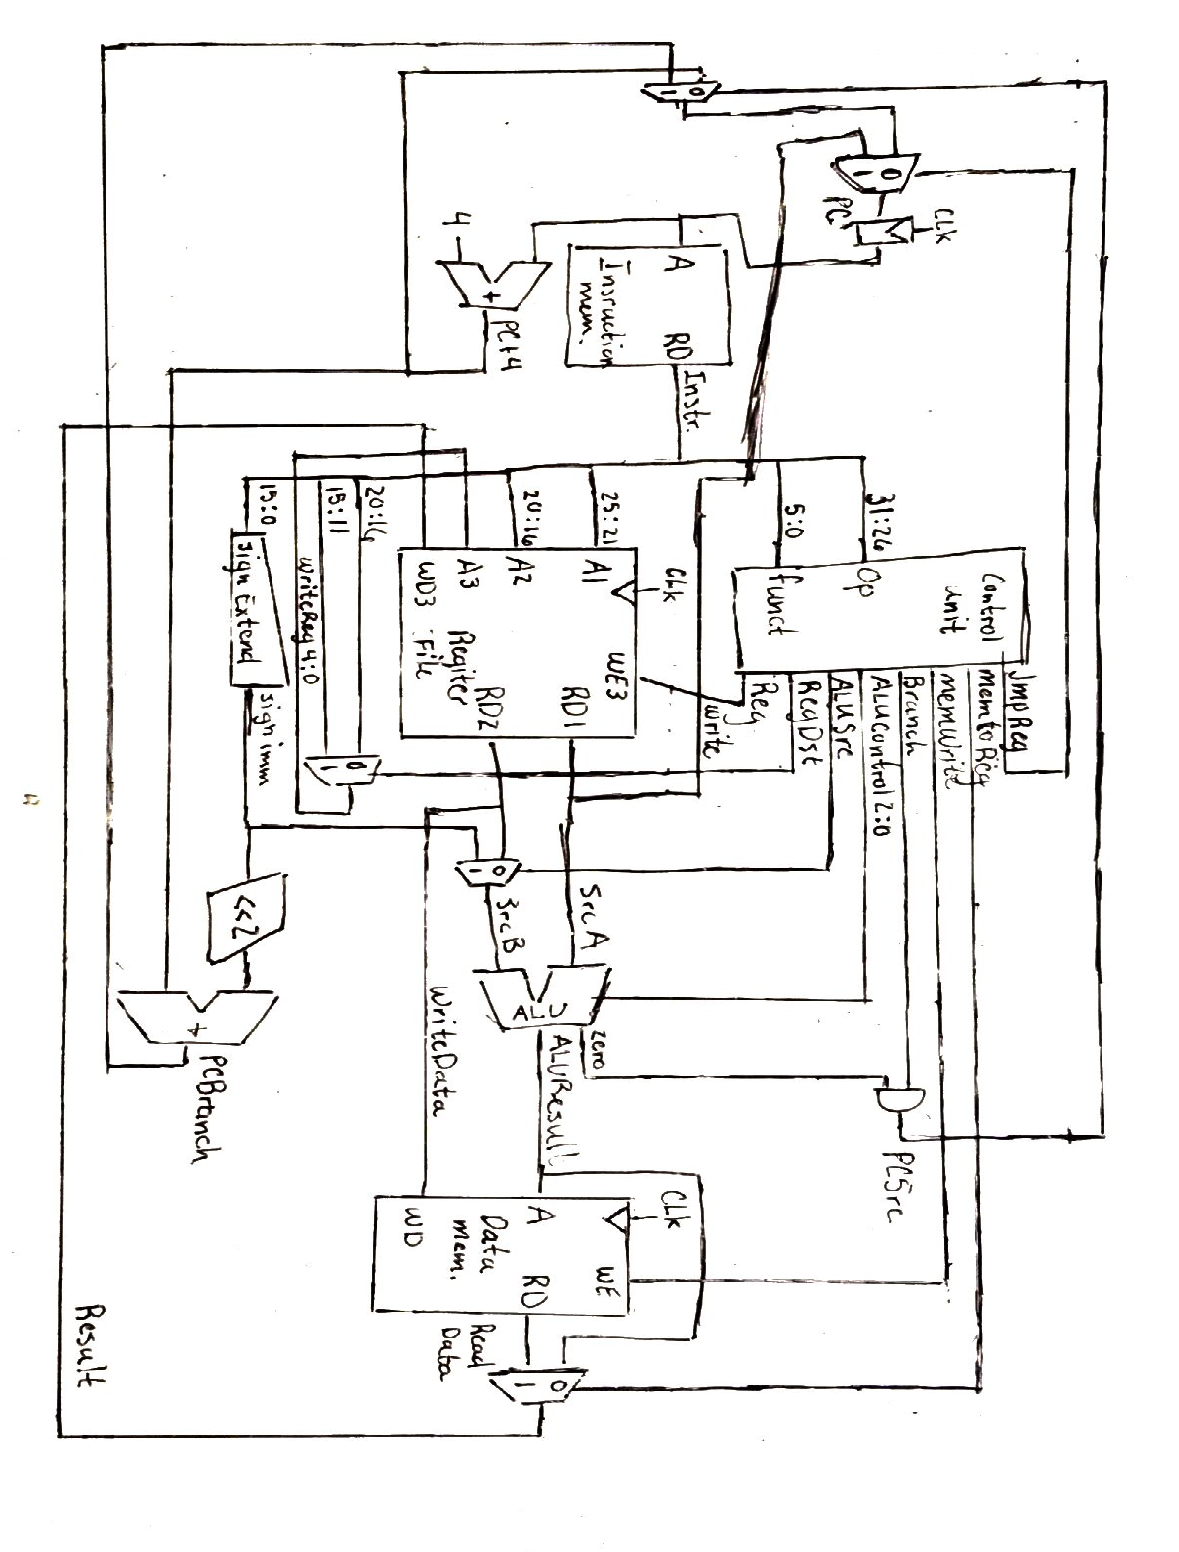
\includegraphics[angle=90,origin=c,width=0.8\textwidth]{7_4c}
				\caption{MIPS single-cycle processor with \texttt{jr} instruction.}
				\label{fig:7_4c}
			\end{figure}
			\begin{table}[h!]
                                \noindent\makebox[\textwidth]{
                                \begin{tabular}{| c c c c c c c c c |}
                                \hline
                                Instruction & Opcode & RegWrite & RegDst & ALUSrc & Branch & MemWrite & MemtoReg & ALUOp\\
                                \hline
                                \hline
                                R-Type & 000000 & 1 & 1 & 0 & 0 & 0 & 0 & 10\\
                                \hline
                                \texttt{lw} & 100011 & 1 & 0 & 1 & 0 & 0 & 1 & 00\\
                                \hline
                                \texttt{sw} & 101011 & 0 & X & 1 & 0 & 1 & X & 00\\
                                \hline
                                \texttt{beq} & 000100 & 0 & X & 0 & 1 & 0 & X & 01\\
                                \hline
                                \texttt{jr} & 001000 & 0 & 1 & 0 & 0 & 0 & X & 00\\
                                \hline
                                \end{tabular}
                                }
                        \caption{Decoder truth table for \texttt{jr} instruction.}
                        \label{tab:jr_truth_table}
                        \end{table}
			\pagebreak
		\item Your friend is a crack circuit designer. She has offered to redesign one
			of the units in the single-cycle MIPS processor to have half the delay.
			Using the delays from Table \ref{tab:delays}, which unit should she
			work on to obtain the greatest speedup of the overall processor, and
			what would the cycle time of the improved machine be?\\
			\begin{equation}
				T_c=t_{pcq\_\text{PC}}+2t_{\text{mem}}+t_{RF\text{read}}+t_{\text{ALU}}+t_{\text{mux}}+t_{RF\text{setup}}
				\label{eq:cycle_time}
			\end{equation}
			The element with the highest delay is \texttt{memory read $t_{\text{mem}}$}
			with 250 ps if this is reduced to 125 ps then following Equation 
			\ref{eq:cycle_time} the cycle time will be:
			\begin{align*}
				T_c_1 &= 30 + 2\left( 125 \right) + 150 + 200 + 25 + 20\\
				T_c_1 &= 685 \text{ ps}
			\end{align*}
			
		\item Suppose that one of the following control signals in the single-cycle
			MIPS processor has a \textit{stuck-at-0 fault}, meaning that the
			signal is always $0$, regardless of its intended value. What
			instructions would malfunction? Why?
			\begin{enumerate}
				\item \textit{RegWrite}:\\
					No register will be written in the Register File. All
					R-Type instructions with destination register \texttt{rd},
					and I-Type instructions with destination register
					\texttt{rt} wont be able to write.
				\item $ALUOp_1$:\\
					ALU will perform addition so branch outcomes might 
					be faulty.
				\item \textit{MemWrite}:\\
					Store word \texttt{sw} will not work properly because there
					will be no writing to memory.
			\end{enumerate}
			
	\end{enumerate}
\clearpage
	\begin{figure}[ht!]
		\centering
		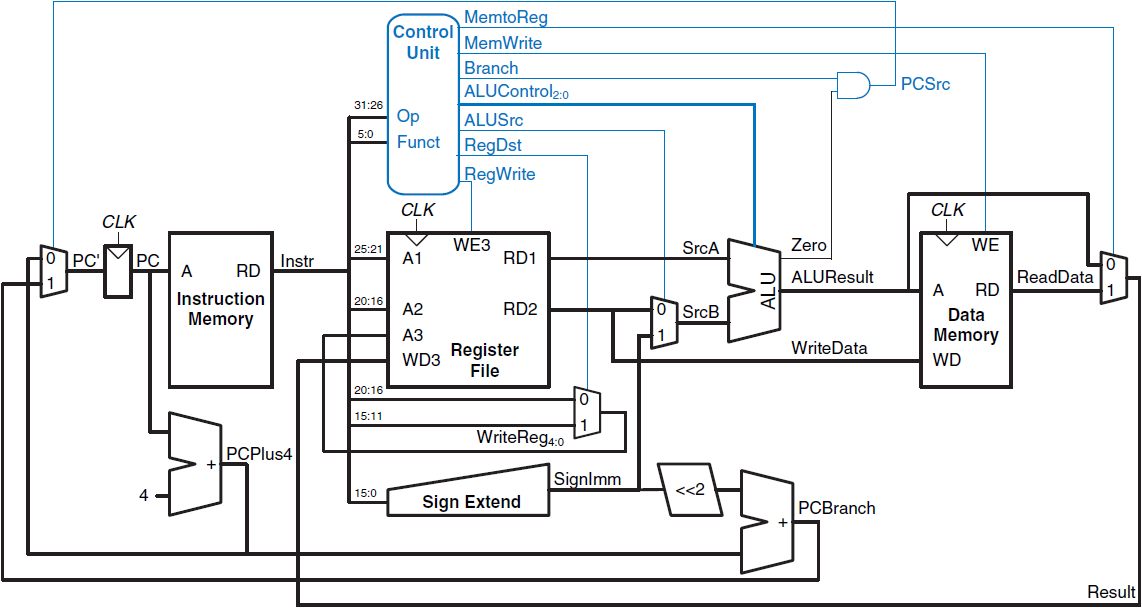
\includegraphics[width=\textwidth]{single_cycle_mips_processor}
		\caption{Complete single cycle MIPS processor}
		\label{fig:1cycle_processor}
	\end{figure}

	\begin{table}[ht]
	\noindent\makebox[\textwidth]{
		\begin{tabular}{| c c c c c c c c c |}
			\hline
			Instruction & Opcode & RegWrite & RegDst & ALUSrc & Branch & MemWrite & MemtoReg & ALUOp\\
			\hline
			\hline
			R-Type & $000000$ & $1$ & $1$ & $0$ & $0$ & $0$ & $0$ & $10$\\
			\hline
			\texttt{lw} & $100011$ & $1$ & $0$ & $1$ & $0$ & $0$ & $1$ & $00$ \\
			\hline
			\texttt{sw} & $101011$ & $0$ & X & $1$ & $0$ & $1$ & X &  $00$ \\
			\hline
			\texttt{beq} & $000100$ & $0$ & X & $0$ & $1$ & $0$ & X & $01$ \\
			\hline
		\end{tabular}
		%\caption{Main decoder truth table to mark up with changes}
		%\label{tab:dec_truth_table}
	}
	\caption{Main decode truth table to mark up with changes}
	\label{tab:dec_truth_table}
	\end{table}

	\begin{table}[ht]
		\centering
		\begin{tabular}{| c c c |}
			\hline
			Element & Parameter & Delay (ps)\\
			\hline
			\hline
			register clk-to-Q & $t_{pcq}$ & $30$ \\
			\hline
			register setup & $t_{\text{setup}}$ & $20$ \\
			\hline
			multiplexer & $t_{\text{mux}}$ & $25$ \\
			\hline
			ALU & $t_{\text{ALU}}$ & $200$ \\
			\hline
			memory read & $t_{\text{mem}}$ & $250$ \\
			\hline
			register file read & $t_{RF\text{read}}$ & $150$\\
			\hline
			register file setup & $t_{RF\text{setup}}$ & $20$ \\
			\hline
		\end{tabular}
		\caption{Delays of circuit elements}
		\label{tab:delays}
	\end{table}

\end{document}
